
\begin{appendices}

\chapter{IQ Demodulation}
IQ demodulation is a major part in the receiver processing of radar data. After going through the mixing process, the signal can be expressed as \citep{lee_1991}
\begin{equation}
\label{eq:signal}
	x_R(t)=A(t)\sin(f_t t+\theta(t)).
\end{equation}
Here, $f_t$ is the carrier frequency of the transmitted pulse. The goal of IQ demodulation is to extract $A(t)$ and $\theta(t)$ from \eqref{eq:signal}, as well as getting rid of the carrier frequency dependency. At the end, a complex signal of the form $A(t)e^{i\theta(t)}$ is obtained.

Most classical radars follow the demodulation scheme depicted in figure \ref{fig:iq_demod}. The first step is to split the signal in \eqref{eq:signal} into two separate channels. In the upper channel, the signal is multiplied by a sinusoid which is generated with the same carrier frequency as the received pulse. The result of this multiplication can be rewritten as
\begin{gather}
	 A(t)\sin(f_t t+\theta(t))\cdot 2\sin(f_t t) = \\
	\label{eq:split}
 	 A(t)\cos(\theta(t))-A(t)\cos(2f_t t+\theta(t)).
\end{gather}
The next step in the demodulation scheme is to low pass filter the signal. Thus, the high frequency term in \eqref{eq:split} is removed, and only $A(t)\cos(\theta(t))$ remains. We define this as $I(t)$.

Similarly, in the bottom channel in figure \ref{fig:iq_demod}, the original signal is multiplied by a generated wave signal of the same carrier frequency. However, this time, the signal is shifted 90 degrees in phase. Similar to before, we may rewrite the product as
\begin{gather}
	 A(t)\sin(f_t t+\theta(t))\cdot 2\cos(f_t t) = \\
	\label{eq:split2}
 	 A(t)\sin(\theta(t))+A(t)\sin(2f_t t+\theta(t)).
\end{gather}
After low pass filtering we obtain $A(t)\sin(\theta(t))$, which we define as $Q(t)$. Finally, by defining $I$ and $Q$ as the real- and imaginary parts of a complex number, respectively, we have our IQ-data
\begin{equation}
	I(t)+iQ(t)=A(t)\Big(\cos(\theta(t))+i\sin(\theta(t))\Big)=A(t)e^{i\theta(t)}
\end{equation}

\begin{figure}
	\centering
	\hbox{\hspace{-0.5em} 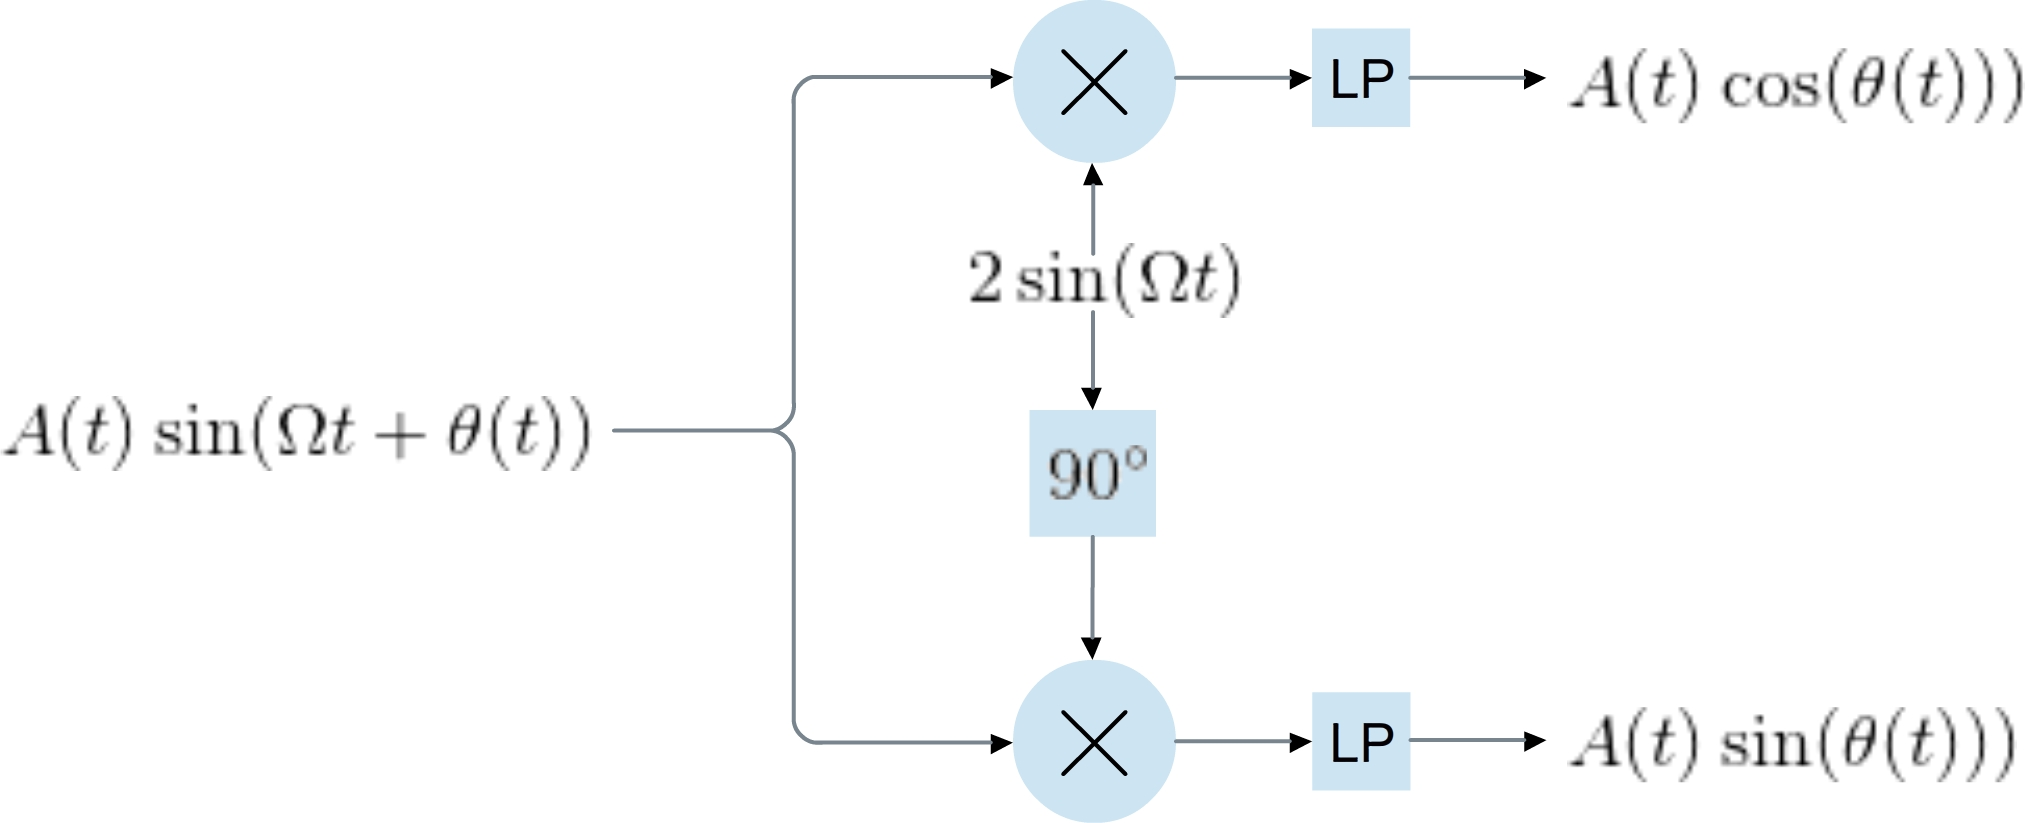
\includegraphics[scale=0.60]{figs_temp/iq_demod.jpg}}
	\caption{Schematics for a typical IQ demodulation.}
	\label{fig:iq_demod}
\end{figure}

% ######### MIXING PROOF ##########
\chapter{Proof of \ref{eq:n1} and \ref{eq:n2}}

For signals $r(t)$ and $x(t)$ defined as

\begin{equation}
	\begin{split}
		r(t) &= CA(t - D)\sin(\Omega(t - D)) \\
		x(t) &= A(t)\sin(\Omega t) \\
	\end{split}
\end{equation}
with angular frequency $\Omega = 2\pi f_t$, where $A(t)$ is the defined as 

\begin{equation}
	A(t) = \begin{cases}
		1 & \text{if $0 \leq t < L$} \\
		0 & \text{otherwise}
	\end{cases}
\end{equation}
the output of the mixing process becomes

\begin{equation}
	m(\tau) 
	= \int_{-\infty}^{+\infty}r(t)x(t-\tau)dt
\end{equation}

\begin{equation}	
	= C \int_{-\infty}^{+\infty}A(t-D)A(t-\tau)\sin(\Omega(t-D))\sin(\Omega(t-\tau))dt.
\end{equation}

This integral can be split into three cases:

\begin{enumerate}[label=(\roman*)]
	\item When $|\tau-D| \geq L$, i.e. when no overlap occurrs. 
	\item When $|\tau-D| < L$ and $\tau \leq D$.
	\item When $|\tau-D| < L$ and $\tau > D$.
\end{enumerate}

The first case, (i), clearly results in the integral becoming 0. Case (ii) can be written as

\begin{equation}
	m(\tau)
	= C\int_{D}^{\tau+L}\sin(\Omega(t-D))\sin(\Omega(t-\tau))dt
\end{equation}

\begin{equation}
	= \frac{C}{2}\int_D^{\tau+L} \cos(\Omega(\tau-D)) - \cos(\Omega(2t - D - \tau))dt
\end{equation}

\begin{equation}
	= \frac{C}{2}\Big( (\tau+L-D)\cos(\Omega(D-\tau)) 
	- \frac{1}{2\Omega}\Big[ \sin(\Omega(2t-D-\tau) \Big]_{D}^{\tau+L} \Big)
\end{equation}

\begin{equation}\label{eq:long}
	= \frac{C}{2}\Big((\tau + L - D)\cos(\Omega(D-\tau))
	- \frac{1}{2\Omega}\big(
	\sin(\Omega(\tau + 2L - D))
	- \sin(\Omega(D-\tau))
	\big)\Big)
\end{equation}

Selecting $L$ as a whole number $n$ of wavelengths $\lambda$, the argument of the second sinusoid can be simplified into

\begin{equation}
	\Omega(\tau + 2L - D) 
	= \Omega(\tau - D) + 2\frac{2\pi f n\lambda}{c} 
\end{equation}

\begin{equation}
	= \Omega(\tau - D) + 2\frac{2\pi f n c}{c f}
	= \Omega(\tau - D) + 4\pi n.
\end{equation}

This means that, as the sinus function is odd functions and periodic in $2\pi$, \ref{eq:long} can be rewritten as 

\begin{equation}\label{eq:first}
	 \frac{C}{2}\Big( (\tau+L-D)\cos(\Omega(\tau - D)) 
	- \frac{1}{\Omega}\sin(\Omega(\tau - D))\Big).
\end{equation}

For (iii), we get a similar integral differing in the integral limits

\begin{equation}
	m(\tau) 
	= \int_\tau^{D+L}\sin(\Omega(t-D))\sin(\Omega(t-\tau))dt
\end{equation}

which is calculated similarly to (ii) to yield

\begin{equation}\label{eq:latter}
	\frac{C}{2}\Big( (D + L - \tau)\cos(\Omega(\tau - D))
	+ \frac{1}{\Omega}\sin(\Omega(\tau - D))\Big).
\end{equation}

Thus, the full mixing output can be written as

\begin{equation}
	m(\tau) = \begin{cases}
		0 & \text{if $|\tau-D|\geq L$} \\
		\text{(\ref{eq:first})} & \text{if $|\tau-D| < L$ and $\tau \leq D$} \\
		\text{(\ref{eq:latter})} & \text{if $|\tau-D| < L$ and $\tau>D$}.
	\end{cases}
\end{equation}

\end{appendices}


